\documentclass[openany]{book}

\usepackage[margin=1in]{geometry}
\usepackage{amsmath,amsfonts,amsthm, amssymb}
\usepackage{yhmath}
\usepackage{mathrsfs}
\usepackage{mathtools}
\usepackage{xcolor}
\usepackage{graphicx}
\usepackage{comment}
\usepackage{tikz-cd}
\usepackage{quiver}
\renewcommand{\familydefault}{ppl}
\newcommand{\tr}{\text{tr}}
\newcommand{\R}{\mathbb{R}}
\newcommand{\E}{\mathbb{E}}
\newcommand{\Z}{\mathbb{Z}}
\newcommand{\C}{\mathbb{C}}
\newcommand{\F}{\mathbb{F}}
\newcommand{\la}{\langle}
\newcommand{\ra}{\rangle}
\newcommand{\colim}{\text{colim}}
\DeclareMathOperator{\im}{im}
\let\oldemptyset\emptyset
\let\emptyset\varnothing
\newcommand{\tor}{\text{Tor}}
\newcommand{\id}{\text{id}}
\newcommand{\ext}{\text{Ext}}
\newcommand{\ptop}{\text{PTop}}
\newcommand{\pt}{\text{pt}}
\newcommand{\ach}{\text{Ach}}
\newcommand{\Q}{\mathbb{Q}}
\newcommand{\gal}{\text{Gal}}


\usepackage{thmtools,thm-restate}

% Fixing mdframed skip below
% See https://tex.stackexchange.com/a/292090/143086
\usepackage[framemethod=TikZ]{mdframed}
\usepackage{xpatch}
\makeatletter
\xpatchcmd{\endmdframed}
	{\aftergroup\endmdf@trivlist\color@endgroup}
	{\endmdf@trivlist\color@endgroup\@doendpe}
	{}{}
\makeatother

\definecolor{huilightpink}{HTML}{fff2fe}
\definecolor{huidarkpink}{HTML}{d955b7}
\declaretheoremstyle[
	mdframed={
		backgroundcolor=huilightpink,
		linecolor=huidarkpink,
		rightline=false,
		topline=false,
		bottomline=false,
		linewidth=2pt,
		innertopmargin=5pt,
		innerbottommargin=8pt,
		innerleftmargin=8pt,
		leftmargin=-2pt,
		skipbelow=2pt,
		nobreak
	},
	headfont=\normalfont\bfseries\color{huidarkpink}
]{huipinkbox}
\declaretheorem[style=huipinkbox,name=Theorem,within=chapter]{thm}
\declaretheorem[style=huipinkbox,name=Theorem,sibling=thm]{theorem}




\begin{comment}
\definecolor{huilightyellow}{HTML}{fff5d6}
\definecolor{huidarkyellow}{HTML}{fcad03}
\declaretheoremstyle[
	mdframed={
		backgroundcolor=huilightyellow,
		linecolor=huidarkyellow,
		rightline=false,
		topline=false,
		bottomline=false,
		linewidth=2pt,
		innertopmargin=5pt,
		innerbottommargin=8pt,
		innerleftmargin=8pt,
		leftmargin=-2pt,
		skipbelow=2pt,
		nobreak
	},
	headfont=\normalfont\bfseries\color{huidarkyellow}
]{huiyellowbox}
\declaretheorem[style=huiyellowbox,name=Proposition,within=chapter]{prop}
\end{comment}



\definecolor{huilightpurple}{HTML}{faf2ff}
\definecolor{huidarkpurple}{HTML}{912ed9}
\declaretheoremstyle[
	mdframed={
		backgroundcolor=huilightpurple,
		linecolor=huidarkpurple,
		rightline=false,
		topline=false,
		bottomline=false,
		linewidth=2pt,
		innertopmargin=5pt,
		innerbottommargin=8pt,
		innerleftmargin=8pt,
		leftmargin=-2pt,
		skipbelow=2pt,
		nobreak
	},
	headfont=\normalfont\bfseries\color{huidarkpurple}
]{huipurplebox}
\declaretheorem[style=huipurplebox,name=Proposition,within=chapter]{prop}



% \definecolor{huilightpurple}{HTML}{faf2ff}
% \definecolor{huidarkpurple}{HTML}{912ed9}
% \declaretheoremstyle[
% 	mdframed={
% 		backgroundcolor=huilightpurple,
% 		linecolor=huidarkpurple,
% 		rightline=false,
% 		topline=false,
% 		bottomline=false,
% 		linewidth=2pt,
% 		innertopmargin=5pt,
% 		innerbottommargin=8pt,
% 		innerleftmargin=8pt,
% 		leftmargin=-2pt,
% 		skipbelow=2pt,
% 		nobreak
% 	},
% 	headfont=\normalfont\bfseries\color{huidarkpurple}
% ]{huipurplebox}
\declaretheorem[style=huipurplebox,name=Lemma,within=chapter]{lem}


\definecolor{lightpink}{HTML}{f0f6fc}
\definecolor{darkpink}{HTML}{2c72b8}
\declaretheoremstyle[
	mdframed={
		backgroundcolor=lightpink,
		linecolor=darkpink,
		rightline=false,
		topline=false,
		bottomline=false,
		linewidth=2pt,
		innertopmargin=5pt,
		innerbottommargin=8pt,
		innerleftmargin=8pt,
		leftmargin=-2pt,
		skipbelow=2pt,
		nobreak
	},
	headfont=\normalfont\bfseries\color{darkpink}
]{pinkbox}
\declaretheorem[style=pinkbox,name=Definition,within=chapter]{defn}


\definecolor{huilightblue}{HTML}{edf9ff}
\definecolor{huidarkblue}{HTML}{4b79db}
\declaretheoremstyle[
	mdframed={
		backgroundcolor=huilightblue,
		linecolor=huidarkblue,
		rightline=false,
		topline=false,
		bottomline=false,
		linewidth=2pt,
		innertopmargin=5pt,
		innerbottommargin=8pt,
		innerleftmargin=8pt,
		leftmargin=-2pt,
		skipbelow=2pt,
		nobreak
	},
	headfont=\normalfont\bfseries\color{huidarkblue}
]{huiblueblox}
\declaretheorem[style=huiblueblox,name=Example,within=chapter]{example}



% \definecolor{huilightblue}{HTML}{edf9ff}
% \definecolor{huidarkblue}{HTML}{4b79db}
% \declaretheoremstyle[
% 	mdframed={
% 		backgroundcolor=huilightblue,
% 		linecolor=huidarkblue,
% 		rightline=false,
% 		topline=false,
% 		bottomline=false,
% 		linewidth=2pt,
% 		innertopmargin=5pt,
% 		innerbottommargin=8pt,
% 		innerleftmargin=8pt,
% 		leftmargin=-2pt,
% 		skipbelow=2pt,
% 		nobreak
% 	},
% 	headfont=\normalfont\bfseries\color{huidarkblue}
% ]{huiblueblox}
% \declaretheorem[style=huiblueblox,name=Example,within=chapter]{example}

% \declaretheoremstyle[
% 	mdframed={
% 		backgroundcolor=huilightblue,
% 		linecolor=huidarkblue,
% 		rightline=false,
% 		topline=false,
% 		bottomline=false,
% 		linewidth=2pt,
% 		innertopmargin=5pt,
% 		innerbottommargin=8pt,
% 		innerleftmargin=8pt,
% 		leftmargin=-2pt,
% 		skipbelow=2pt,
% 		nobreak
% 	},
% 	headfont=\normalfont\bfseries\color{huidarkblue}
% ]{huiblueblox}
\declaretheorem[style=huiblueblox,name=Problem,within=chapter]{prob}



% \declaretheoremstyle[
% 	mdframed={
% 		backgroundcolor=huilightblue,
% 		linecolor=huidarkblue,
% 		rightline=false,
% 		topline=false,
% 		bottomline=false,
% 		linewidth=2pt,
% 		innertopmargin=5pt,
% 		innerbottommargin=8pt,
% 		innerleftmargin=8pt,
% 		leftmargin=-2pt,
% 		skipbelow=2pt,
% 		nobreak
% 	},
% 	headfont=\normalfont\bfseries\color{huidarkblue}
% ]{huiblueblox}
\declaretheorem[style=huiblueblox,name=Exercise,within=chapter]{exer}
\declaretheorem[style=huipinkbox, name=Corollary, within=chapter]{cor}





















\newcommand{\nirwarnsymbol}{%
	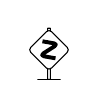
\begin{tikzpicture}[baseline=(x.base)]
		\draw[rounded corners=.01em] (-.05em,-1.07em)rectangle(.05em,.78em);
		\draw[fill=white,rounded corners=1.3] (0,.75em)--(.75em,0)--(0,-.75em)--(-.75em,0)--cycle;
		\draw[line width=0.2mm, line cap=round](-.4em,-1.07em)--(.4em,-1.07em);
		\node(x) at (0,0em) {};
		% Thank you https://tex.stackexchange.com/a/262510
		\draw[
			line cap=but,
			line join=round,
			x=.5em,
			line width=0.5mm,
			y=1*(height("Z")-\pgflinewidth)*(1-sin(10)),
			rotate=-10,
			rounded corners=1.5pt,
		](-0.57, 0.57) -- (0.57, 0.57) -- (-0.57, -0.57) -- (0.57, -0.57);
	\end{tikzpicture}%
}

%%%%%%%%%%%%%%%%%%%%%%%%%%%%%%%%%%%%%%%%%%%% MARGINS
\usepackage{marginnote}
% Thank you https://tex.stackexchange.com/a/472882
% Makes marginnotes always appear on the left, apparently
%
\makeatletter
\long\def\@mn@@@marginnote[#1]#2[#3]{%
	\begingroup
		\ifmmode\mn@strut\let\@tempa\mn@vadjust\else
			\if@inlabel\leavevmode\fi
			\ifhmode\mn@strut\let\@tempa\mn@vadjust\else\let\@tempa\mn@vlap\fi
		\fi
		\@tempa{%
			\vbox to\z@{%
				\vss
				\@mn@margintest
				\if@reversemargin\if@tempswa
						\@tempswafalse
					\else
						\@tempswatrue
				\fi\fi

					\llap{%
						\vbox to\z@{\kern\marginnotevadjust\kern #3
							\vbox to\z@{%
								\hsize\marginparwidth
								\linewidth\hsize
								\kern-\parskip
								%\mn@parboxrestore
								\marginfont\raggedleftmarginnote\strut\hspace{\z@}%
								\ignorespaces#1\endgraf
								\vss
							}%
							\vss
						}%
						\if@mn@verbose
							\PackageInfo{marginnote}{xpos seems to be \@mn@currxpos}%
						\fi
						\begingroup
							\ifx\@mn@currxpos\relax\else\ifx\@mn@currpos\@empty\else
									\kern\@mn@currxpos
							\fi\fi
							\ifx\@mn@currpage\relax
								\let\@mn@currpage\@ne
							\fi
							\if@twoside\ifodd\@mn@currpage\relax
									\kern-\oddsidemargin
								\else
									\kern-\evensidemargin
								\fi
							\else
								\kern-\oddsidemargin
							\fi
							\kern-1in
						\endgroup
						\kern\marginparsep
					}%
			}%
		}%
	\endgroup
}
\makeatother
%
% Mostly for todonotes
\renewcommand{\marginpar}{\marginnote}
%%%%%%%%%%%%%%%%%%%%%%%%%%%%%%%%%%%%%%%%%%%% /MARGINS

\definecolor{nirlightred}{RGB}{250, 220, 220}
\definecolor{nirdarkred}{HTML}{f40000}
\declaretheoremstyle[
	mdframed={
		backgroundcolor=nirlightred,
		linecolor=nirdarkred,
		rightline=false,
		topline=false,
		bottomline=false,
		linewidth=2pt,
		innertopmargin=5pt,
		innerbottommargin=8pt,
		innerleftmargin=8pt,
		leftmargin=-2pt,
		skipbelow=2pt,
		nobreak
	},
	headfont=\normalfont\bfseries\color{nirdarkred}
]{nirredbox}

% \makeatletter
% \declaretheorem[
% 	style=nirredbox,
% 	name=Warning,
% 	sibling=thm,
% 	% without \leavevmode, the first item in a list gets misformatted
% 	postheadhook={\leavevmode\marginnote{\nirwarnsymbol}[-3pt]%
% 	\ifthmt@thisistheone% restatable makes alignment weird
% 		\hspace{-2.2pt}%
% 	\fi}
% ]{warn}
% \makeatother

\newcommand{\nirideasymbol}{%
	
\begin{tikzpicture}[baseline=(x.base)]
		\draw[rounded corners=.01em] (-.05em,-1.07em)rectangle(.05em,.78em);
		\draw[fill=white,rounded corners=1.3] (0,.75em)--(.75em,0)--(0,-.75em)--(-.75em,0)--cycle;
		\draw[line width=0.2mm, line cap=round](-.4em,-1.07em)--(.4em,-1.07em);
		\node(x) at (0,0em) {};
		\node at (0,0em) {{\textbf{!}}};
	\end{tikzpicture}%
}
\renewcommand{\nirwarnsymbol}{%
	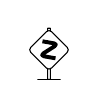
\begin{tikzpicture}[baseline=(x.base)]
		\draw[rounded corners=.01em] (-.05em,-1.07em)rectangle(.05em,.78em);
		\draw[fill=white,rounded corners=1.3] (0,.75em)--(.75em,0)--(0,-.75em)--(-.75em,0)--cycle;
		\draw[line width=0.2mm, line cap=round](-.4em,-1.07em)--(.4em,-1.07em);
		\node(x) at (0,0em) {};
		% Thank you https://tex.stackexchange.com/a/262510
		\draw[
			line cap=but,
			line join=round,
			x=.5em,
			line width=0.5mm,
			y=1*(height("Z")-\pgflinewidth)*(1-sin(10)),
			rotate=-10,
			rounded corners=1.5pt,
		](-0.57, 0.57) -- (0.57, 0.57) -- (-0.57, -0.57) -- (0.57, -0.57);
	\end{tikzpicture}%
}
\makeatletter
\declaretheorem[
	style=nirredbox,
	name=Idea,
	sibling=thm,
	% without \leavevmode, the first item in a list gets misformatted
	postheadhook={\leavevmode\marginnote{\nirideasymbol}[-3pt]%
	\ifthmt@thisistheone% restatable makes alignment weird
		\hspace{-2.2pt}%
	\fi}
]{idea}

\declaretheorem[
	style=nirredbox,
	name=Warning,
	sibling=thm,
	% without \leavevmode, the first item in a list gets misformatted
	postheadhook={\leavevmode\marginnote{\nirwarnsymbol}[-3pt]%
	\ifthmt@thisistheone% restatable makes alignment weird
		\hspace{-2.2pt}%
	\fi}
]{warn}
\makeatother

\title{Algebra Qualifying Exam Solutions
\\ 
\vspace{0.4cm}
\Large (Accuracy Not Guaranteed)}




\date{\today}
\author{Hui Sun}


\begin{document}

\maketitle

\tableofcontents
\newpage


\begin{warn}
    I cannot do Nakayama lemma questions.
\end{warn}


\textcolor{blue}{Fall 2019, Spring 2018}


\chapter{Fall 2019}

\textcolor{red}{3,5}

\begin{prob}
    Let \(\mathbb{F}_{q}\) be a field with \(q\neq 9\) elements and \(a\) be a generator of the cyclic group \(\mathbb{F}^{*}_{q}\). Show that \(\mathrm{SL}_{2}(\mathbb{F}_{q})\) is generated by
    \[\left(\begin{array}{cc}1&1\\0&1\end{array}\right),\ \left(\begin{array}{cc}1&0\\a&1\end{array}\right).\]
\end{prob}
\begin{proof}
    I will not do all the computation here, but here are a list of matrices one can get using these generators:
    \begin{equation*}
        \begin{pmatrix}
            1&t\\
            0&1
        \end{pmatrix}, \quad \begin{pmatrix}
            1&0\\
            1&1
        \end{pmatrix},\quad \begin{pmatrix}
            0&-1\\
            1&0
        \end{pmatrix}
    \end{equation*}
    where $t$ is any element in $\F_q$. And one can essentially show that these generate all the upper triangular matrices in $\text{SL}_2(\F_q)$, i.e.,
    \begin{equation*}
        \left\{\begin{pmatrix}
            x&y\\
            0&x^{-1}
        \end{pmatrix}: x,y\in\F_q\right\}
    \end{equation*}
    and one can show that any matrix in $\text{SL}_2(\F_q)$ is a product of $\begin{pmatrix}
        0&-1\\
        1&0
        \end{pmatrix} $ and upper triangular matrices, then done.
\end{proof}




\begin{prob}
    Let \(p,q\) be two prime numbers such that \(p|q-1\). Prove that:
    \begin{itemize}
        \item[(a)] there exists an integer \(r\not\equiv 1\mod q\) such that \(r^{p}\equiv 1\mod q\);
        \item[(b)] there exists (up to an isomorphism) only one noncommutative group of order \(pq\).
    \end{itemize}
\end{prob}
\begin{proof}
    \begin{itemize}
        \item[(a)] We want to find there exists $r\in (\Z/q\Z)^\times$ such that $r\neq 1$ such that $r^p\equiv 1\mod q$. If $p\mid(q-1)$, then there exists an element of order $p$ in the group $(\Z/q\Z)^\times$ by Cauchy's theorem, i.e., $r^{p}\equiv 1\mod q$.
        \item[(b)] We must have $q>p$ then $n_q=1$, and we can write 
        \begin{equation*}
            G=N\otimes_\theta P
        \end{equation*}
        where $N$ is a normal $q$-subgroup and $P$ is a Sylow $p$-subgroup. We note that 
        \begin{equation*}
            \theta: 1\mapsto r
        \end{equation*}
        where $r$ is an element of order $p$, which exists by (a). And the group is described as 
        \begin{equation*}
            G=\la g,h: g^q=h^p=e: hgh^{-1}=g^{r}\ra
        \end{equation*}
        This group is unique because the elements $g\mapsto g^r$ where $r$ is any element wth order $p$ forms a subgroup in $\text{Aut}(\Z/q\Z)$, thus they define isomorphic strucutres of $G$.
    \end{itemize}
\end{proof}


\begin{prob}
    Let \(F,L\) be extensions of a field \(K\). Suppose that \(F/K\) is finite. Show that there exists an extension \(E/K\) such that there are monomorphisms of \(F\) into \(E\) and of \(L\) into \(E\) which are identical on \(K\).
\end{prob}



\begin{prob}
    Find all irreducible representations of a finite \(p\)-group over a field of characteristic \(p\).
\end{prob}
\begin{proof}
    Let $G$ any finite $p$-group. Let $V$ be an irreducible representation over $\F_p$, consider the $[\F_pG]$-module $W$ generated by any $v\in V\setminus\{0\}$. We see $W$ is a finite-dimensional vector space over $\F_p$, i.e., 
    \begin{equation*}
        |W|=p^d
    \end{equation*}
    for some $d\geq 1$. We consider the action of $G$ on $W$, all the orbits of this action either has size $1$ or is a power of $p$, since $G$ is a $p$-group, by the class formula, let $N$ be the number of nontrivial orbits of size $1$, 
    \begin{equation*}
        |W|\equiv 1+N\mod p\Rightarrow 1+N\equiv 0\mod p
    \end{equation*}
    Hence there exists at least one nontrivial orbit $\{v\}$ of size $1$. We consider the vector space $\bar{W}$ generated by $v$ over $\F_p$: it is one-dimensional vector space contained in $V$, invariant under $G$, since $V$ is irreducible, we must have $V=\bar{W}$. The action of $G$ on $\bar{W}$ is the trivial action, thus all irreducible representations of a finite $p$-group over $\F_p$ are trivial.
\end{proof}


\begin{prob}
    How many two-sided ideals has the group algebra \(\mathbb{C}[\mathrm{S}_{3}]\), where \(\mathrm{S}_{3}\) is the group of permutations of \(\{1,2,3\}\)?
\end{prob}




\chapter{Spring 2018}


\textcolor{red}{1,2,3,5}

\begin{prob}
    Let \(F\) be a field of characteristic not equal to 2. Let \(D\) be the non-commutative algebra over \(F\) generated by elements \(i,j\) that satisfy the relations
    \[i^2 = j^2 = 1, \quad ij = -ji.\]
    Define \(k = ij.\)
    \begin{itemize}
        \item[(a)] Verify that \(D\) is isomorphic to the algebra \(M_2(F)\) of \(2 \times 2\) matrices in such a way that
        \[1 \leftrightarrow \begin{pmatrix} 1 & 0 \\ 0 & 1 \end{pmatrix}, i \leftrightarrow \begin{pmatrix} 1 & 0 \\ 0 & -1 \end{pmatrix}, j \leftrightarrow \begin{pmatrix} 0 & 1 \\ 1 & 0 \end{pmatrix}, k \leftrightarrow \begin{pmatrix} 0 & 1 \\ -1 & 0 \end{pmatrix}.\]
        \item[(b)] Write \(q = x + yi + zj + uk\) for \(x,y,z,u \in F\). Verify that the norm
        \[N(q) = x^2 - y^2 - z^2 + u^2\]
        corresponds to the determinant under the isomorphism of part (a).
        \item[(c)] What does the involution \(q \mapsto \bar{q} = x - yi - zj - uk\) on \(D\) correspond to on the matrix side?
    \end{itemize}
\end{prob}




\begin{prob}
    Let \(R\) be a commutative ring. An \(R\)-module \(M\) is said to be finitely presented if there exists a right-exact sequence
    \[R^m \longrightarrow R^n \longrightarrow M \longrightarrow 0\]
    for some non-negative integers \(m,n\). Prove that any finitely generated projective \(R\)-module \(P\) is finitely presented.
\end{prob}





\begin{prob}
    Let \(R\) be the ring \(\mathbb{Z}[\zeta_p]\), where \(p\) is a prime number and \(\zeta_p\) denotes a primitive \(p\)th root of unity in \(\mathbb{C}\). Prove that if an integer \(n \in \mathbb{Z}\) is divisible by \(1 - \zeta_p\) in \(R\), then \(p\) divides \(n\).
\end{prob}




\begin{prob}
    Is \(S_4\) isomorphic to a subgroup of \(\text{GL}_2(\mathbb{C})\)?
\end{prob}
\begin{proof}
    We've done this in Spring 2017 exam. We want to show there is no injective homomorphism from $S_4$ to $\text{GL}_2(\C)$, i.e., it is a representation. The $2$ dimensional representation and the direct sum of $1$-dimensional representations all send $(12)(34)$ to $\begin{pmatrix}
        1&0\\
        0&1
    \end{pmatrix}$.
\end{proof}




\begin{prob}
    Let \(n\) be a positive integer and \(A\) an abelian group. Prove that
    \[\text{Ext}^1(\mathbb{Z}/n\mathbb{Z}, A) \cong A/nA.\]
\end{prob}





\chapter{Fall 2017}


\begin{prob}
    Show that there is no simple group of order 30.
\end{prob}
\begin{proof}
    We know that $n_5=1$ or $6$, if $n_5=1$, then we are done. If $n_5=6$, then there are $30-4\cdot 6=6$ elements of order $\neq 6$, and we know there exists at least one Sylow $2$-subgroup and one Sylow $3$-subgroup, combined with the identity element, we see either $n_2=1$ or $n_3=1$. 
\end{proof}


\begin{prob}
    Let \(\Lambda\) be a free abelian group of finite rank \(n\), and let \(\Lambda^{\prime}\subset\Lambda\) be a subgroup of the same rank. Let \(x_{1},\ldots,x_{n}\) be a \(\mathbb{Z}\)-basis for \(\Lambda\), and let \(x^{\prime}_{1},\ldots,x^{\prime}_{n}\) be a \(\mathbb{Z}\)-basis for \(\Lambda^{\prime}\). For each \(i\), write \(x^{\prime}_{i}=\sum_{j=1}^{n}a_{ij}x_{j}\), and let \(A:=(a_{ij})\in \text{Mat}_{n\times n}(\mathbb{Z})\). Show that the index \([\Lambda:\Lambda^{\prime}]\) equals \(|\det A|\).
\end{prob}
\begin{proof}
    We notice that $\Lambda=\Z\oplus\dots\oplus\Z$, and $\Lambda'$ is a subgroup of same rank thus 
    \begin{equation*}
        \Lambda'=d_1\Z\oplus\dots\oplus d_n\Z
    \end{equation*}
    where $d_i$ are integers, up to some basis change (we will argue below why change of basis doesn't affect the equality). We note that 
    \begin{equation*}
        [\Lambda:\Lambda']=\left|\prod_{i=1}^nd_i\right|
    \end{equation*}
    It suffices to take the basis of $\Lambda$ as $x_i=(0,\dots,0,1,0,\dots,0)$, where only the $i$th entry is nonzero and equal to $1$, and the basis for $\Lambda'$ as $x_j'=(0,\dots, 0,d_j,0,\dots, 0)$, where only the $j$th entry is nonzero and equal to $d_j$. This is because for any change of basis matrix $P$, we have 
    \begin{equation*}
        \det(PAP^{-1})=\det(A)
    \end{equation*} 
    i.e., we can freely change the basis of $A$. With respect to the basis chosen above, we have 
    \begin{equation*}
        A=\begin{pmatrix}
            d_1&0&\dots&0\\
            0&d_2&\dots&0\\
            \dots&\dots&\dots&\dots\\
            0&\dots&\dots&d_n
        \end{pmatrix}
    \end{equation*}
    This shows that 
    \begin{equation*}
        \left|\det A\right|=\left|\prod_{i=1}^nd_i\right|=[\Lambda:\Lambda']
    \end{equation*}
    as desired.
\end{proof}


\begin{prob}
    In this problem all rings are commutative.
    \begin{itemize}
        \item[(a)] Let \(R\) be a local ring with maximal ideal \(\mathfrak{m}\), let \(N\) and \(M\) be finitely generated \(R\)-modules, and let \(f\colon N\to M\) be an \(R\)-linear map. Show that \(f\) is surjective if and only if the induced map \(N/\mathfrak{m}N\to M/\mathfrak{m}M\) is.
        \item[(b)] Recall that a module \(M\) over a ring \(R\) is \textit{projective} if the functor \(\operatorname{Hom}_{R}(M,-)\) is exact. Show that if \(R\) is local and \(M\) is finitely generated projective, then \(M\) is free.
    \end{itemize}
\end{prob}
\begin{proof}
    \begin{itemize}
        \item[(a)] If $f$ is surjective, this means for any $y\in M$ there exists $x$ such that $f(x)=y$, hence the induced map $\overline{f}: x+\mathfrak{m}N\mapsto f(x)+\mathfrak{m}M$ is also sujrective: for any $y+\mathfrak{m}M$ there exists $x+\mathfrak{m}M$ such that $\overline{f}(x+\mathfrak{m}M)=y+\mathfrak{m}M$. Conversely, consider $\im(f)\subset M$, since $\overline{f}$ is surjective, we have $M=\im(f)+\mathfrak{m}M$, by Nakayama's lemma, 
        \begin{equation*}
            \mathfrak{m}(M/\im(f))=0
        \end{equation*}
        implies that $M/\im(f)=0$, i.e., $M=\im(f)$.
        
        
        
        
        % \)take any $y\in M$, we know there exists $x$ such that $y-f(x)\in \mathfrak{m}M$
        \item[(b)] I give up.
    \end{itemize}
\end{proof}



\begin{prob}
    Compute the Galois group of \(x^{5}-10x+5\) over \(\mathbb{Q}\).
\end{prob}
\begin{proof}
    One can graph this function and see there are only $3$ real roots, we first note 
    \begin{equation*}
        \begin{cases}
            f(-2)<0\\
            f(-1)>0\\
            f(1)<0\\
            f(2)>0
        \end{cases}
    \end{equation*}
    By IVT, there are at least $3$ real roots. By Rolle's theorem, between any roots, there must exists a point $f'(c)=0$, therefore we argue there can be at most 3 real roots because there are only two points $p$ such that $f'(p)=0$. This shows that there are $2$ complex roots, and let $r_1$ be a complex root. By Eisenstein, this polynomial is irreducible, and we know the Galois group $G$ is a subgroup of $S_5$. Because $G$ contains a transposition (sending two complex roots to each other), and an element of order $5$, we know that $G$ must be equal to $S_5$.

    % , therefore a real root $r_2$ has minimal polynomial degree $5$ i.e., the Galois extension has degree 
    % \begin{equation*}
    %     \Q\subset\Q(r_1)\subset\Q(r_1,r_2)
    % \end{equation*}
    % has degree $125$. Since it contains an element of order $2$ (permuting the two complex roots) and and order $5$, the Galois group must be $S_5$.
\end{proof}




\begin{prob}
    Let \(K/k\) be an extension of finite fields with \(\#k=q\), let \(\Phi\colon x\mapsto x^{q}\) denote the \(q\)th power Frobenius map on \(K\), and let \(G:=\text{Gal}(K/k)\).
    \begin{itemize}
        \item[(a)] Compute the minimal polynomial of \(\Phi\) as a \(k\)-linear endomorphism of \(K\).
        \item[(b)] Use (a) to prove the \textit{normal basis theorem} in the case of the extension \(K/k\): there exists \(x\in K\) such that the set \(\{\sigma x\mid\sigma\in G\}\) is a \(k\)-basis for \(K\).
    \end{itemize}
\end{prob}
\begin{proof}
    \begin{itemize}
        \item[(a)] Let $|K|=q^n$, we claim that the minimal polynomial is $f(t)=t^n$. This is because $\Phi$ is a generator of $G$, and $G$ has order $n$. (One can prove this fact by assuming there exists some $k<n$ such that $x^{p^k}=x$ for all $x\in K$, then $q^n$ divides $q^k$, which is a contradiction).
        \item[(b)] We will use some general fact about linear algebra: $T:V\to V$ is a linear map, the minimal polynomial is equal to the characteristic polynomial if and only if there exists a vector $v$ such that  $\{v, Tv,\dots, T^{n-1}v\}$ is a basis for $V$. By (a), we know the minimal polynomial coincide with the characteristic polynomial, since $G$ is cyclic with generator $\Phi$, we see that there exists $x$ such that
        \begin{equation*}
            \left\{x,\Phi x,\dots, \Phi^{n-1}x\right\}
        \end{equation*}
        is a basis for $K$ over $k$.
    \end{itemize}
\end{proof}


\begin{prob}
    Let \(G\) be a finite group with center \(Z\subset G\). Show that if \(G\) admits a faithful irreducible representation \(G\to\text{GL}_{n}(k)\) for some positive integer \(n\) and some field \(k\), then \(Z\) is cyclic.
\end{prob}
\begin{proof}
    We first assume that $k$ is algebraically closed. We know that $\rho(z)$ is a $G$-invariant map: take any $g\in G$,
    \begin{equation*}
        \rho(z)(\rho(g)(v))=\rho(g)\rho(z)(v)
    \end{equation*}
    therefore $\rho(z)=\lambda I_n$ for some $\lambda\in k^\times$, this shows that $\rho$ embdes $z$ into a group of $k^\times$, i.e., a cyclic group.

    Now for the case where $k$ is not algebraically closed. Then any $\rho\otimes k^a$ is also faithful, and although $\rho\otimes k^a$ might not be irreducible, if $\rho\otimes k^a=\rho_1+\rho_2$, where $\rho_i$ are irreducible, then it follows that both $\rho_1$ and $\rho_2$ are faithful representations of $G$ over $k^a$. This again shows that $Z$ is cyclic.
\end{proof}







\chapter{Spring 2017}


\begin{prob}
    Let \(A\) be a commutative ring, and define the \textit{nilradical} \(\sqrt{0}\) to be the set of nilpotent elements in \(A\). Show that \(\sqrt{0}\) is equal to the intersection of all prime ideals in \(A\). Show that if \(A\) is reduced, then \(A\) can be embedded into a product of fields.
\end{prob}
\begin{proof}
    Let $\{P_i:i\in I\}$ be the collection of prime ideals in $A$. We first show that 
    \begin{equation*}
        \sqrt{0}=\bigcap_{i}P_i
    \end{equation*}
    Let $a\in\sqrt{0}$, then for some $n\geq 0$, $a^n=0$, this implies that for all $i\in I$,
    \begin{equation*}
        a^n\in P_i\Rightarrow a\in P_i \text{ or } a^{n-1}\in P_i
    \end{equation*}
    since $P_i$ is prime. We claim that $a\in P_i$. If not, then $a^{n-1}\in P_i$ which implie $a^{n-2}\in P_i$ $\dots$ which eventually implies $a\in P_i$, which is a contradiction. Hence $\sqrt{0}\subset \bigcap_iP_i$. Now for the reverse inclusion, we use the following lemma:
    \begin{lem}
        Let $S$ be a multiplicative set in $A$ such that $0\not\in S$, then there exists a prime ideal $P\subset A$ such that 
        \begin{equation*}
            S\cap P=\emptyset
        \end{equation*}
    \end{lem}
    Let $a\in\bigcap_iP_i$, then the set 
    \begin{equation*}
        S=\{a, a^2, \dots\}
    \end{equation*}
    is a multiplicative set, suppose that $a$ is not nilpotent, i.e., $a\not\in S$, then there exists a prime ideal that does not interserct $S$, which is a contradiction since $a\in P_i$ for all $i$. Thus 
    \begin{equation*}
        \sqrt{0}=\bigcap_iP_i
    \end{equation*}

    Now we show that if $A$ is reduced, then $A$ can be embedded into a product of fields. If $A$ is reduced, then $\sqrt{0}=0$, i.e., if $a\neq0$, then $a$ cannot be in all the prime ideals. Suppose $a\neq 0$, then there exists some $P_i$ such that $a\not\in P_i$. Then we can consider the map 
    \begin{equation*}
        A\to \frac{A}{P_i}\to\text{Frac}\left( \frac{A}{P_i}\right)
    \end{equation*}
    where 
    \begin{equation*}
        a\mapsto a+P_i\mapsto \frac{a+P_i}{1}
    \end{equation*}
    Thus we claim that $A$ embeds in 
    \begin{equation*}
        A\xrightarrow{\iota}\text{Frac}\left( \frac{A}{P_1}\right)\times \text{Frac}\left( \frac{A}{P_2}\right)\times\dots=\prod_{i\in I}\text{Frac}\left( \frac{A}{P_i}\right)
    \end{equation*}
    where $\text{Frac}$ denotes the field of fractions. If $a=0$, then $\iota(a)=(0,\dots, 0)$, if $a\neq 0$, then $a\not\in P_j$ for some $j$, and 
    \begin{equation*}
        \iota(a)=\left(0,\dots, 0, \frac{a+P_j}{1},0,\dots, 0\right)
    \end{equation*}
    where only the $j$-th entry is nonzero.
\end{proof}



\begin{prob}
    Write down the minimal polynomial for \(\sqrt{2}+\sqrt{3}\) over \(\mathbb{Q}\) and prove that it is reducible over \(\mathbb{F}_{p}\) for every prime number \(p\).
\end{prob}
\begin{proof}
    The minimal polynomial $p_m$ is 
    \begin{equation*}
        p_m(t)=(t^2-5)^2-24=t^4-10t^2+1
    \end{equation*}
    The roots are $\pm\sqrt{2}\pm\sqrt{3}$, thus this polynomial generates a field extension of $\Q$, 
    \begin{equation*}
        \Q(\sqrt{2},\sqrt{3})=\frac{\Q[t]}{(p_m(t))}
    \end{equation*}
    We claim that it suffices to show that $\sqrt{2}$ or $\sqrt{3}$ or $\sqrt{6}$ are in $\F_p$ for any prime $p$. Take $\sqrt{2}\in\F_p$ for example, we know $p_m(t)$ is not irreducible over $\Q(\sqrt{2})$, because then it would mean the degree of field extension $[\Q(\sqrt{2},\sqrt{3}): \Q]$ is 8, which is a contradiction.
    \[\begin{tikzcd}
        {\mathbb{Q}(\sqrt{2},\sqrt{3})} \\
        {\mathbb{Q}(\sqrt{2})} \\
        {\mathbb{Q}}
        \arrow[from=2-1, to=1-1]
        \arrow[from=3-1, to=2-1]
    \end{tikzcd}\]
    Thus $p_m(t)$ is reducible over $\Q(\sqrt{2})$. Now we show the following.
    \begin{lem}
        For any prime $p$, $\sqrt{2}$ or $\sqrt{3}$ or $\sqrt{6}$ are in $\F_p$ for any prime $p$.
    \end{lem}
    There exists a homomorphism (Legendre symbol) $\varphi:\F_p^\times\to \{\pm 1\}$, such that 
    \begin{equation*}
        \varphi(g)=\begin{cases}
            1, \text{ if $g$ is a square}\\
            -1, \text{ otherwise}
        \end{cases}
    \end{equation*}
    Suppose that $2,3$ are not squares, i.e., $sqrt{2},\sqrt{3}\not\in\F_p^\times$, then 
    \begin{equation*}
        \varphi(2\cdot 3)=1
    \end{equation*}
    which implies $\sqrt{6}\in\F_p^\times$, concluding the proof.
\end{proof}

\begin{prob}
    Let \(K/k\) be a finite separable field extension, and let \(L/k\) be any field extension. Show that \(K\otimes_{k}L\) is a product of fields.
\end{prob}
\begin{proof}
    We know $K/k$ implies there exists $\alpha\in K$ such that 
    \begin{equation*}
        K=k(\alpha)
    \end{equation*}
    moreover, for any $t\in K$, the minimal polynomial of $t$ factors into distinct linear factors. Let $p_\alpha$ be the minimal polynomial of $\alpha$, 
    \begin{align*}
        K\otimes_kL&=\frac{k[t]}{(p_\alpha(t))}\otimes_kL\\
        &=\frac{L[t]}{(p_\alpha(t))}\\
        &=\frac{L[t]}{(p_\alpha^1(t))\dots(p_\alpha^k(t))}
    \end{align*}
    where $p_\alpha^i(t)$ are distinct irreducible factors over in $L[t]$. By Chinese Remainder Theorem, we must have 
    \begin{equation*}
        K\otimes_kL=\frac{L[t]}{(p_\alpha^1(t))}\dots\frac{L[t]}{(p_\alpha^k(t))}
    \end{equation*}
    i.e., a product of fields.
\end{proof}


\begin{prob}
    Let \(M\) be an invertible \(n\times n\) matrix with entries in an algebraically closed field \(k\) of characteristic not 2. Show that \(M\) has a square root, i.e. there exists \(N\in\text{Mat}_{n\times n}(k)\) such that \(N^{2}=M\).
\end{prob}
\begin{proof}
    It suffices to show that every Jordan block 
    \[
        J_n(\lambda) = 
        \begin{bmatrix}
        \lambda & 1       & 0       & \cdots & 0 \\
        0       & \lambda & 1       & \cdots & 0 \\
        0       & 0       & \lambda & \ddots & \vdots \\
        \vdots  & \vdots  & \ddots  & \ddots & 1 \\
        0       & 0       & \cdots  & 0      & \lambda
        \end{bmatrix}
        \]
        where $\lambda\neq 0$ is a square. We will proceed using inductino. When $n=2$, the square root of 
        \begin{equation*}
            \begin{bmatrix}
                \lambda&1\\
                0&\lambda
            \end{bmatrix}=\begin{bmatrix}
                \lambda^\frac{1}{2}&\frac{1}{2}\lambda^{-\frac{1}{2}}\\
                0&\lambda^\frac{1}{2}
            \end{bmatrix}^2
        \end{equation*} 
        Now assume that $J_{k}$ is a square up to $k=n-1$, we want to show $J_n$ also has a square root. We claim $J_n$ has the following square 
        \begin{equation*}
            J_n=\begin{bmatrix}
                B^2&x\\
                0&\lambda

            \end{bmatrix}=\begin{bmatrix}
                B&x\\
                0&\lambda^{1/2}
            \end{bmatrix}^2
        \end{equation*}
        where $B$ is a $(n-1)\times (n-1)$ matrix and $x=(x_1,\dots,x_{n-1}), 0=(0,\dots,0)$. It suffices to find such an $x$ exists. Let $b_1,\dots,b_{n-1}$ denote the row vectors of $B$, we must satisfy 
        \begin{equation*}
            \begin{cases}
                b_1\cdot x+x_1\lambda^\frac{1}{2}=0\\
                \dots\\
                b_{n-2}\cdot x+x_{n-2}\lambda^\frac{1}{2}=0\\
                b_{n-1}\cdot x+x_{n-1}\lambda^\frac{1}{2}=1\\
            \end{cases}
        \end{equation*}
        Namely, we need to find $x$ that satisfies 
        \begin{equation*}
            (B+\lambda^\frac{1}{2}I)x=\begin{bmatrix}
                0\\
                \dots\\
                0\\
                1
            \end{bmatrix}
        \end{equation*}
        Since $(B+\lambda^{1/2}I)$ is invertible, there exists a unique solution, hence such $x$ exsits, $J_n$ has a square root!
\end{proof}



\begin{prob}
    Prove directly from the definition of (left) semisimple ring that every such ring is (left) Noetherian and Artinian. (You may freely use facts about semisimple, Noetherian, and Artinian modules.)
\end{prob}
\begin{proof}
    If $R$ is Artinian, then $R$ can be decomposed into a finite sum of simple rings, let $R_1,\dots, R_n$ be simple rings, we can write 
    \begin{equation*}
        R=\bigoplus_{i=1}^nR_i
    \end{equation*}
    where $R_i$ contains only the trivial ideal and $R_i$ as ideals. Now it is quite clear that every ascending and descending chain of ideals stabilizes because there are only finitely many distinct ideals. 
\end{proof}

\begin{prob}
    Let \(G\) be a finite group and \(H\) an abelian subgroup. Show that every irreducible representation of \(G\) over \(\mathbb{C}\) has dimension \(\leq[G:H]\).
\end{prob}
\begin{proof}
    Any irreduicble representation $\rho:H\to\mathbb{C}^\times$ is one-dimensional, and we consider induced representation of $\rho$, $\text{Ind}_H^G\rho$, we note that $\text{Ind}_H^G\rho$ is not necessarily irreducible, hence for any irreducible representation $\tilde{\rho}:G\to\text{GL}_n(\C)$, we have 
    \begin{equation*}
        \dim\tilde{\rho}\leq\dim(\text{Ind}_H^G\rho)
    \end{equation*}
    and 
    \begin{equation*}
        \text{Ind}_H^G\rho=\bigoplus_{i=1}^ng_iH
    \end{equation*}
    where $g_i$ are the representatives of the coset and the sum consists of exactly one copy for each coset. Hence we see 
    \begin{equation*}
        \dim\tilde{\rho}\leq\dim(\text{Ind}_H^G\rho)=[G:H]
    \end{equation*}
\end{proof}




\chapter{Fall 2016}



\begin{prob}
    Determine \(\text{Aut}(S_{3})\).
\end{prob}
\begin{proof}
    $\sigma\in\text{Aut}(S_3)$ is determined by where $(12)$ and $(123)$ are sent to. There are $6$ options in total and all of them are homomorphisms (conjugation). It is easy to check that this group is not commutative, i.e., 
    \begin{equation*}
        \text{Aut}(S_3)\cong S_3
    \end{equation*}
\end{proof}

\begin{prob}
    A group \(G\) is a semidirect product of subgroups \(N,H\subset G\) if \(N\) is normal and every element of \(G\) has a unique presentation \(nh\), \(n\in N\), \(h\in H\). Find all semidirect products (up to isomorphism) of \(N=\mathbb{Z}/11\mathbb{Z}\), \(H=\mathbb{Z}/5\mathbb{Z}\).
\end{prob}
\begin{proof}
    Let $G=N\rtimes_\theta H$, where 
    \begin{equation*}
        \theta: \Z/5\Z\to \text{Aut}(\Z/11\Z)\cong\Z/10\Z
    \end{equation*}
    such that
    \begin{equation*}
        5\theta(1)\equiv 0\mod 10
    \end{equation*}
    Thus $\theta(1)$ could be $0, 2,4,6,8$. When $\theta(1)=0$, this gives the abelian group 
    \begin{equation*}
        G\cong\frac{\Z}{5\Z}\times\frac{\Z}{11\Z}
    \end{equation*}
    We claim that all nontrivial $\theta$ give rise to the same semidirect product, namely, the following diagram commutes
    \[\begin{tikzcd}
        {\Z/5\Z} & {\Z/10\Z} \\
        {\Z/5\Z} & {\Z/10\Z}
        \arrow["{\theta'}", from=1-1, to=1-2]
        \arrow["m"', from=1-1, to=2-1]
        \arrow["{\text{id}}", from=1-2, to=2-2]
        \arrow["\theta", from=2-1, to=2-2]
    \end{tikzcd}\]
    for $\theta: 1\mapsto 2$ and any $\theta': 1\mapsto 4, 6, 8$, by taking $m$ to be the multiplication map by $2,3,4$ respectively. Hence we see 
    \begin{equation*}
        \theta(h)(g)=g^{2^{2h}}
    \end{equation*}
    by observing 
    \[\begin{tikzcd}
        {\Z/5\Z} & {\Z/10\Z} & {\left(\Z/11\Z\right)^\times} & {\text{Aut}(\Z/11\Z)}
        \arrow["2", from=1-1, to=1-2]
        \arrow["{2^2}", from=1-2, to=1-3]
        \arrow["{2^2\cdot(-)}"', from=1-3, to=1-4]
    \end{tikzcd}\]
    In other words,
    \begin{equation*}
        G=\left\la g,h: g^{11}=h^5=1, hgh^{-1}=g^{4}\right\ra
    \end{equation*}
\end{proof}

\begin{prob}
    Let \(F\) be a finite field of order \(2^{n}\). Here \(n>0\). Determine all values of \(n\) such that the polynomial \(x^{2}-x+1\) is irreducible in \(F[x]\).
\end{prob}
\begin{proof}
    We know that $x^2-x+1$ is irreducible over $\F_2$, namely, it has no roots in $\F_2$. Since there is only one field of order $4$, we must have 
    \begin{equation*}
        \F_4\cong\frac{\F_2}{(x^2-x+1)}
    \end{equation*}
    Clearly $x^2-x+1$ is not irreducible over $\F_4$. For any $\F_{2^n}$, we know $(x^2-x+1)$ is irreducible if and only if $\F_4$ does not embed into $\F{2^n}$, i.e., $2\nmid n$. This shows that when $n$ is odd, the polynomial $x^2-x+1$ is irreducible over $\F_{2^n}$.
\end{proof}

\begin{prob}
    \begin{itemize}
        \item[(1)] Determine the Galois group of \(x^{4}-4x^{2}-2\) over \(\mathbb{Q}\).
        \item[(2)] Let \(G\) be a group of order 8 such that \(G\) is the Galois group of a polynomial of degree 4 over \(\mathbb{Q}\). Show that \(G\) is isomorphic to the Galois group in part (1).
    \end{itemize}
\end{prob}
\begin{proof}
    \begin{itemize}
        \item[(1)] The roots of this polynomial is $\pm\sqrt{2\pm\sqrt{6}}$, and notice that 
        \begin{equation*}
            \sqrt{2}i=\sqrt{2+\sqrt{6}}\sqrt{2-\sqrt{6}}
        \end{equation*}
        This gives the splitting field (Galois extension) of this polynomila as 
        \begin{equation*}
            \Q\left(\sqrt{2+\sqrt{6}}, \sqrt{2}i\right)
        \end{equation*}
        We see that 
        \begin{equation*}
            \Q\left(\sqrt{2+\sqrt{6}}\right)\cap\Q(\sqrt{2}i)=\emptyset
        \end{equation*}
        because the first is contained in $\R$ and the second is not. We must have 
        \begin{equation*}
            \left[ \Q\left(\sqrt{2+\sqrt{6}}, \sqrt{2}i\right)/\Q\right]=8
        \end{equation*}
        By part b, we see $\text{Gal}\cong D_8$.
        \item[(2)] Any Galois group of a polynomial with $4$ roots in the splitting field embeds into $S_4$, and we notice that $|G|=2^3, |S_4|=2^3\cdot 3$, i.e., $G$ is a Sylow $2$-subgroup of $S_4$, and all Sylow $2$-subgroups are conjugate/isomorphic of one another, hence 
        \begin{equation*}
            \text{Gal}\cong D_8
        \end{equation*}
    \end{itemize}
\end{proof}

\begin{prob}
    Let A be a linear transformation of a finite dimensional vector space over a field of characteristic \(\neq 2\).
    \begin{itemize}
        \item[(1)] Define the wedge product linear transformation \(\wedge^{2}A=A\wedge A\).
        \item[(2)] Prove that
        \[tr(\wedge^{2}A)=\frac{1}{2}(tr(A)^{2}-tr(A^{2})).\]
    \end{itemize}
\end{prob}
\begin{proof}
    (Recall we have analogous results for $A\otimes A$).
    \begin{itemize}
        \item[(1)] The wedge product $A\wedge A$ is defined on the wedge product of vector spaces $V\wedge V$, so we first define the vector space: let $\{v_1,\dots, v_n\}$ be the basis of $V$, then $\{v_i\wedge v_j\}$ where $i<j$ forms a basis of $V\wedge V$, satisfying:
        \begin{enumerate}
            \item $v_i\wedge v_j=-v_j\wedge v_i$
            \item $(a_iv_i+a_jv_j)\wedge (b_kv_k+b_lv_l)=(a_ib_k)v_i\wedge v_k+(a_ib_l)v_i\wedge v_l+(a_jb_k)v_j\wedge v_k+(a_jb_l)v_j\wedge v_l$
        \end{enumerate}
        And $A\wedge A$ where $A:V\to V$ is defined as 
        \begin{equation*}
            A\wedge A(v_i\wedge v_j)=Av_i\wedge Av_j
        \end{equation*}
        \item[(2)] Consider the matrix representation of $A=(A_{ij})$, on the basis $\{v_i\wedge v_j: i<j\}$, 
        \begin{align*}
            A\wedge A(v_i\wedge v_j)&=\sum_{k,l=1}^nA_{ki}A_{lj}(v_k\wedge v_l)\\
            &=\sum_{k<l}A_{ki}A_{lj}(v_k\wedge v_l)+\sum_{l<k}A_{ki}A_{lj}(v_k\wedge v_l)\\
            &=\sum_{k<l}A_{ki}A_{lj}(v_k\wedge v_l)-\sum_{l<k}A_{ki}A_{lj}(v_l\wedge v_k)
        \end{align*}
        Thus the diagonal term with respect to $v_i\wedge v_j$ is 
        \begin{equation*}
            A_{ii}A_{jj}-A_{ji}A_{ij}
        \end{equation*}
        Thus 
        \begin{equation*}
            \text{Tr}(A\wedge A)=\sum_{i<j}A_{ii}A_{jj}-A_{ji}A_{ij}
        \end{equation*}
        Now 
        \begin{equation*}
            \text{Tr}(A)^2=\sum_{i=1}^nA_{ii}^2+2\sum_{i<j}A_{ii}A_{jj}
        \end{equation*}
        and 
        \begin{align*}
            \text{Tr}(A^2)&=\sum_{k,l=1}^nA_{lk}A_{kl}\\
            &=\sum_{i=1}^nA_{ii}^2+2\sum_{k<l}A_{lk}A_{kl}
        \end{align*}
        Thus we see that 
        \[tr(\wedge^{2}A)=\frac{1}{2}(tr(A)^{2}-tr(A^{2}))\]
    \end{itemize}

\end{proof}

\begin{prob}
    Find a table of characters for the alternating group \(A_{5}\).
\end{prob}
\begin{proof}
    \[
\begin{array}{c|ccccc}
 & \text{1} & \text{20} & \text{15} & \text{12} & \text{12} \\ 
 & \text{Id} & (1\,2\,3) & (1\,2)(3\,4) & (1\,2\,3\,4\,5) & (1\,2\,3\,5\,4) \\ 
\hline
\chi_1 & 1 & 1 & 1 & 1 & 1 \\ 
\chi_2 & 3 & 0 & -1 & \phi & 1-\phi \\ 
\chi_3 & 3 & 0 & -1 & 1-\phi & \phi \\ 
\chi_4 & 4 & 1 & 0 & -1 & -1 \\ 
\chi_5 & 5 & -1 & 1 & 0 & 0 \\ 
\end{array}
\]
where $\phi=\frac{1+\sqrt{5}}{2}$.
\end{proof}


\chapter{Spring 2016}

\textcolor{red}{I can't do 6}

\begin{prob}
    Classify all groups of order 66, up to isomorphism.
\end{prob}
\begin{proof}
    There are a total of $4$ groups. We have $n_{11}=1$, take any Sylow-$3$ subgroup, we can construct a subgroup of order $33$ by taking the semidirect product.
    \begin{lem}
        Let $H$ be a subgroup of $G$ such that $[G:H]=p$ is the smallest prime dividing $|G|$, then $H$ is normal.
    \end{lem}
    Using the lemma, we know this subgroup $N$ of order $33$ must be normal and isomorphic to $\Z/33\Z$. Take any Sylow $2$-subgroup of $G$, we know 
    \begin{equation*}
        G=\frac{\Z}{33\Z}\rtimes_\theta \frac{\Z}{2\Z}
    \end{equation*}
    where $\theta: P_2\to\text{Aut}(N)=(\Z/33\Z)^\times$ satisfies 
    \begin{equation*}
        2\theta(1)\equiv 1\mod 33
    \end{equation*}
    We see there are four numbers in $(\Z/33\Z)^\times$ that satisfy this:
    \begin{equation*}
        \theta(1)\mapsto \{1, 10, 23, 32\}
    \end{equation*}
    When $\theta(1)=1$, 
    \begin{equation*}
        G_1\cong\frac{\Z}{33\Z}\times\frac{\Z}{2\Z}
    \end{equation*}
    When $\theta(1)=10$, then 
    \begin{equation*}
        G_2=\la g,h: g^{33}=h^2=1, hgh^{-1}=g^{10}\ra
    \end{equation*}
    When $\theta(1)=23$, we have 
    \begin{equation*}
        G_3=\la g,h: g^{33}=h^2=1, hgh^{-1}=g^{23}\ra
    \end{equation*}
    When $\theta(1)=32$, we have 
    \begin{equation*}
        G_4=\la g,h: g^{33}=h^2=1, hgh^{-1}=g^{32}\ra
    \end{equation*}
\end{proof}


\begin{prob}
    Let \(F\subset K\) be an algebraic extension of fields. Let \(F\subset R\subset K\) where \(R\) is a \(F\)-subspace of \(K\) with the property such that \(\forall a\in R\), \(a^{k}\in R\) for all \(k\geq 2\).
    \begin{itemize}
        \item[(1)] Assume that \(\text{char}(F)\neq 2\). Show that \(R\) is a subfield of \(K\).
        \item[(2)] Give an example such that \(R\) may not be a field if \(\text{char}(F)=2\).
    \end{itemize}
\end{prob}
\begin{proof}
    I will only do (1), because I can't do (2). It suffices to show that $R$ is closed under multiplication and taking inverses. Let $a,b\in R$, we know 
    \begin{equation*}
        (a+b)^2\in R\Rightarrow a^2+b^2+2ab\in R\Rightarrow ab\in R
    \end{equation*}
    Since $F\subset K$ is algebraic, for any $a\in R$, there exists a minimal polynomial $p_a(t)$ such that 
    \begin{equation*}
        p_a(a)=c_0+c_1a+\dots+c_na^n=0
    \end{equation*}
    Multiplying both sides by $a^{-n}$ and equating we get 
    \begin{equation*}
        c_0a^{-n}+\dots+c_n=c_0+c_1a+\dots+c_na^n
    \end{equation*} 
    i.e., 
    \begin{equation*}
        c_0a^{-n}=c_0+c_1a+\dots+c_na^n-c_n-\dots-c_1a^{-(n-1)}
    \end{equation*}
    multiplying both sides by $a^{n-1}$, we see that $a^{-1}\in R$, as desired.
\end{proof}

\begin{prob}
    Determine the Galois group of \(x^{6}-10x^{3}+1\) over \(\mathbb{Q}\).
\end{prob}
\begin{proof}
    Solving for the roots we see the splitting field for this polynomial is 
    \begin{equation*}
        \Q(\sqrt{5+2\sqrt{6}},\sqrt{3}i)
    \end{equation*}
    which has degree $12$, i.e., the order of the Galois group. Let 
    \begin{equation*}
        \begin{cases}
            \alpha_1=\sqrt{5+2\sqrt{6}}\\
            \beta_1=\sqrt{5-2\sqrt{6}}\\
            \alpha_2=e^\frac{2\pi i}{3}\sqrt{5+2\sqrt{6}}\\
            \beta_2=e^\frac{2\pi i}{3}\sqrt{5-2\sqrt{6}}\\
            \alpha_3=e^\frac{4\pi i}{3}\sqrt{5+2\sqrt{6}}\\
            \beta_3=e^\frac{4\pi i}{3}\sqrt{5-2\sqrt{6}}
        \end{cases}
    \end{equation*}
    We see that there are two choices for $\alpha_1\mapsto \alpha_i,\beta_j$ for any $i,j$. This gives a group of order $12$ and by drawing a hexagon (or by guessing), one can conclude that this is $D_{12}$.
\end{proof}

\begin{prob}
    Let \(V\) and \(W\) be two finite dimensional vector spaces over a field \(K\). Show that for any \(q>0\),
    \[\bigwedge^{q}(V\oplus W)\cong\sum_{i=0}^{q}(\bigwedge^{i}(V)\otimes_{K}\bigwedge^{q-i}(W)).\]
\end{prob}
\begin{proof}
    Any two finite dimensional vector spaces of the same dimension are isomorphic. Hence, it suffices to show that the dimensions are equal. We will convince ourselves it holds for $q=2$. Let $\{v_1,\dots, v_n\}$ be the basis of $V$, and $\{w_1,\dots,w_k\}$ be the basis of $W$, then we begin with the LHS:
    \begin{equation*}
        \bigwedge^{2}(V\oplus W)
    \end{equation*}
    We note that $V\oplus W$ has basis 
    \begin{equation*}
        \left\{(v_i,w_j):1\leq i\leq n, 1\leq j\leq k\right\}
    \end{equation*}
    So we reenumerate the $n+k$ basis as 
    \begin{equation*}
        \{e_1,\dots, e_{n+k}\}
    \end{equation*}
    Then $\bigwedge^{q}(V\oplus W)$ has basis
    \begin{equation*}
        \left\{ e_i\wedge e_j: i<j\right\}
    \end{equation*}
    There are exactly $1+\dots+(n+k-1)$ basis vectors i.e.,
    \begin{equation*}
        \dim\left(\bigwedge^{2}(V\oplus W)\right)=\frac{(n+k-1)(n+k)}{2}
    \end{equation*}
    As for the RHS: 
    \begin{equation*}
        \dim\left( \sum_{i=0}^{2}(\bigwedge^{i}(V)\otimes_{K}\bigwedge^{2-i}(W))\right)
        \frac{(k-1)k}{2}+nk+\frac{(n-1)n}{2}
    \end{equation*}
    And we observe that two two quantities are equal. Now we do the general case, just like above, 
    \begin{equation*}
        \dim\left(\bigwedge^{q}(V\oplus W)\right)=\binom{n+k}{q}
    \end{equation*}
    And the RHS:
    \begin{equation*}
        \dim\left(\bigwedge^{q-1}(V\oplus W)\wedge (V\oplus W)\right)=\sum_{i=0}^q\binom{n}{i}\binom{k}{q-i}
    \end{equation*}
    and it is clear that these two quantities are equal.
    
    
    % Inductive step: suppose that this is true up to $\bigwedge^{q-1}$. Now 
    % \begin{align*}
    %     \bigwedge^{q}(V\oplus W)&= \bigwedge^{q-1}(V\oplus W)\wedge (V\oplus W)
    % \end{align*}
    % Let's denote the dimension of $ \bigwedge^{q-1}(V\oplus W)$ as $m$, and recall there are $\{e_1,\dots,e_{n+k}\}$ basis vectors for $V\oplus W$, hence we are reenumerate the basis vectors:
    % \begin{equation*}
    %     \{f_1,\dots, f_{n+k+m}
    % \end{equation*}


    % \begin{align*}
    %     \bigwedge^{q}(V\oplus W) \cong  \sum_{i=0}^{q}(\bigwedge^{i}(V)\otimes_{K}\bigwedge^{q-i}(W))
    % \end{align*}


\end{proof}

\begin{prob}
    Prove that a finite dimensional algebra over a field is a division algebra if and only if it does not have zero divisors.
\end{prob}
\begin{proof}
    Recall a finite dimensional algebra is a ring with a field action, and it is a division algebra if every nonzero element $a\in A$ has an $a^{-1}\in A$. We know $A$ does not have a zero divisor if and only if for any $a\in A$, the multiplication map by $a$ is injective. Since $A$ is a finite dimensional vector space as well, an injective map is necessarily surjective, i.e., multiplication by $a$ is surjective, this happens if and only if $a$ is a unit, i.e., $A$ is a division algebra.
\end{proof}


\begin{prob}
    Let \(A\) be a semi-simple finite dimensional algebra over \(\mathbb{C}\), and let \(V\) be a direct sum of two isomorphic simple \(A\)-modules. Find the automorphism group of the \(A\)-module \(V\).
\end{prob}

\chapter{Fall 2014}


\textcolor{red}{2}

\begin{prob}
    \begin{itemize}
        \item[(a)] Let \(S_n\) be the symmetric group (permutation group) on \(n\) objects. Prove that if \(\sigma \in S_n\) is an \(n\)-cycle and \(\tau \in S_n\) is a transposition (i.e., a 2-cycle), then \(\sigma\) and \(\tau\) generate \(S_n\).
        \item[(b)] Let \(f_a(x)\) be the polynomial \(x^5 - 5x^3 + a\). Determine an integer \(a\) with \(-4 \leq a \leq 4\) for which \(f_a\) is irreducible over \(\mathbb{Q}\), and the Galois group of [the splitting field of] \(f_a\) over \(\mathbb{Q}\) is \(S_5\). Then explain why the equation \(f_a(x) = 0\) is not solvable in radicals.
    \end{itemize}
\end{prob}
\begin{proof}
    \begin{itemize}
        \item[(a)] It suffices to assume that the $n$ cycle is $(1\dots n)$ (up to rearranging the terms), and the transposition is $(12)$. One can show that conjugation gives all the transpositions, hence generate $S_n$.
        \item[(b)] Take $a=1$, then $f_a(x)$ is irreducible: it doesn't have a root by the Rational Root Theorem and cannot be factored into lower degree polynomial by term matching. Moreover, we see that $f_a'(x)$ has $3$ roots, by Rolle's theorem, there are at most $4$ real roots, this implies that there exists a complex root $r_1$, and since this has odd degree, it must also exist a real root $r_2$. This shows that there exists an element in the Galois group that has order $5$ and a transposition (sending conjugate complex roots to each other). Thus by (a), since the Galois group is a subgroup of $S_5$, we must have it equal to $S_5$. 
    \end{itemize}
\end{proof}



\begin{prob}
    Let \(R = \mathbb{Q}[X]\), \(I\) and \(J\) the principal ideals generated by \(X^2 - 1\) and \(X^3 - 1\) respectively. Let \(M = R/I\) and \(N = R/J\). Express in simplest terms [the isomorphism type of] the \(R\)-modules \(M \otimes_R N\) and \(\text{Hom}_R(M, N)\). \textbf{Explain.}
\end{prob}
\begin{proof}
    This is tensor product over fields question, finally! We have 
    \begin{align*}
        M\otimes_{\Q[x]}N&=\frac{\Q[x]}{(X^2-1)}\otimes_{\Q[x]}\frac{\Q[x]}{(X^3-1)}\\
        &=\frac{\Q[x]}{\left(\gcd(X^2-1)+(X^3-1)\right)}\\
        &=\frac{\Q[x]}{(x-1)}\\
        &=\Q
    \end{align*}

\end{proof}


\begin{prob}
    Let \(G = S_3\).
    \begin{itemize}
        \item[(a)] Prove that \(G\) has an irreducible complex representation of dimension 2,—call it \(\rho\)—but none of higher dimension.
        \item[(b)] Decompose \(\rho \otimes \rho \otimes \rho\) (as a representation of \(G\)) into a direct sum of irreducible representations.
    \end{itemize}
\end{prob}
\begin{proof}
    \begin{itemize}
        \item[(a)] $S_3$ has three conjugacy classes, i.e., $3$ irreducible representations, the only way to write $|S_3|=6$ as a sum of $3$ squares is $1+1+4$, which implies that there exists a irred rep of dimension $2$, and not any higher.
        \item[(b)] We know that 
        \begin{equation*}
            \chi\left[(\rho\otimes\rho\otimes\rho)(g)\right]=\left(\chi(\rho(g))\right)^3
        \end{equation*}
        Thus with some trial and error, if we want to write 
        \begin{equation*}
            \rho\otimes\rho\otimes\rho=\sum \chi_{\text{triv}}\dots\oplus\chi_{\text{sgn}}\dots \oplus\rho\dots\rho
        \end{equation*}
        Then we need to send 
        \begin{equation*}
            \rho\otimes\rho\otimes\rho(g)=\begin{cases}
                8, g=e\\
                0, g=(12)\\
                -1, g=(123)
            \end{cases}
        \end{equation*}
        Thus we see that 
        \begin{equation*}
            \rho\otimes\rho\otimes\rho=\chi_{\text{triv}}\oplus\chi_{\text{sgn}}\oplus\rho\oplus\rho\oplus\rho
        \end{equation*}
    \end{itemize}
\end{proof}



\begin{prob}
    \begin{itemize}
        \item[(a)] Let \(G\) be a group of order \(p^2q^2\), where \(p\) and \(q\) are distinct odd primes, with \(p > q\). Show that \(G\) has a normal subgroup of order \(p^2\).
        \item[(b)] Can a solvable group contain a non-solvable subgroup? \textbf{Explain.}
    \end{itemize}
\end{prob}
\begin{proof}
    \begin{itemize}
        \item[(a)] $n_p$ can only be $1$ or $q^2$, if $n_p=q^2$, then
        \begin{equation*}
            p\mid (q^2-1)=(q+1)(q-1)
        \end{equation*}
        i.e., $p$ divides $q+1$ or $q-1$, which are both even, which is a contradiction. This implies $n_p=1$.
        \item[(b)] Let $H$ be a subgroup of $G$, where $G$ is solvable. Then there exists a sequence 
        \begin{equation*}
            \{e\}=G_0\subset G_1\subset\dots G_n=G
        \end{equation*}
        such that each $G_i$ is normal in $G_{i+1}$ and $G_{i+1}/G_i$ is abelian/cyclic. If we take 
        \begin{equation*}
            H_i=G_i\cap H
        \end{equation*}
        then one can show that 
        \begin{equation*}
            \{e\}=H_0\subset\dots\subset H_n=H
        \end{equation*}
        is a sequence satisfying the above condition, i.e., $H$ is solvabla.
    \end{itemize}
\end{proof}



\begin{prob}
    \begin{itemize}
        \item[(a)] Prove that every group of order \(p^2\) (\(p\) a prime) is abelian. Then classify such groups up to isomorphism.
        \item[(b)] Give an example of a non-abelian group of order \(p^3\) for \(p = 3\). \textbf{Suggestion}: Represent the group as a group of matrices.
    \end{itemize}
\end{prob}

\begin{proof}
    \begin{itemize}
        \item[(a)] We know any nontrivial $p$-group has a nontrivial center, thus either $Z(G)=p$ or $Z(G)=p^2$. We are done in the latter case. If $Z(G)=p$, then 
        \begin{equation*}
            G/Z(G) \text{is cyclic}
        \end{equation*}
        which implies $G$ is again abelian, hence we must have $Z(G)=p^2$, as desired.
        \item[(b)] The Heisenburg group over $\F_3$.
    \end{itemize}
\end{proof}





\chapter{Fall 2011}

\textcolor{red}{2,5}

\begin{prob}
    \begin{itemize}
        \item[(a)] Let \(G\) be a group of order 5046. Show that \(G\) cannot be a simple group. You may not appeal to the classification of finite simple groups.
        \item[(b)] Let \(p\) and \(q\) be prime numbers. Show that any group of order \(p^2q\) is solvable.
    \end{itemize}
\end{prob}
\begin{proof}
    \begin{itemize}
        \item[(a)] $5046=29^2\cdot 2\cdot 3$, we must have $n_{29}=1$. This shows $G$ is not simple.
        \item[(b)] There are two cases: $p<q$ and $p>q$. When $p<q$, we if $n_{q}=p^2$ then $n_p=1$, thus when $n_p=q$, we have $n_q=1$. In other words, you either have a normal group of order $p^2$ or $q$, and both cases are solvable. When $p>q$, then $n_q=1$, also solvable.
    \end{itemize}
\end{proof}



\begin{prob}
    Consider the special orthogonal group \(G=SO(3,\mathbb{R})\), namely,
    \[G=\{A\in GL(3,\mathbb{R}): A^T A=\mathrm{I}_3, \det(A)=1\}\]
    \begin{itemize}
        \item[(a)] Show that for any element \(A\) in \(G\), there exists a real number \(\alpha\) with \(-1\leq\alpha\leq 3\) such that
        \[A^3-\alpha A^2+\alpha A-\mathrm{I}_3=0.\]
        \item[(b)] For which real numbers \(\alpha\) with \(-1\leq\alpha\leq 3\) does there exist an element \(A\) in \(G\) whose minimal polynomial is \(x^3-\alpha x^2+\alpha x-1\)? Explain your answer.
    \end{itemize}
\end{prob}
\begin{proof}
    This question is quite computational, and I will not list all the computations here.
    \begin{itemize}
        \item[(a)] Writing $A$ in a general form, we see that 
        \begin{equation*}
            \alpha=\text{tr}(A)
        \end{equation*}
        Thus it sufficees to compute the eigenvalues of $A$ (in the algebraic closure). 
    \end{itemize}
    
\end{proof}



\begin{prob}
    Let \(G\) be a cyclic group of order 100. Let \(K=\mathbb{Q}\), the field of rational numbers, or \(K=F_p\), the finite field with \(p\) elements, \(p\) being a prime number. For each such \(K\), construct a Galois extension \(L/K\) whose Galois group \(\text{Gal}(L/K)\) is isomorphic to \(G\). Explain your construction in detail.
\end{prob}
\begin{proof}
    First we do $K=\F_p$. Let $E$ be the splitting field of $(x^{p^{100}}-x)$, then by definition $E$ is Galois, we see $\F_p\subset E$ (so it is an extension) because if $a\in\F_p$,
    \begin{equation*}
        a^p=a\Rightarrow (a^{p^{100}}-a)=0
    \end{equation*}
    Thus $\F_p\subset E$. Now $E$ is a degree $100$ extension of $\F_p$, i.e., $\left|\gal(E/\F_p)\right|=100$. Now by the following lemma, we are done.
    \begin{lem}
        Let $\F_p\subset E=\F_{p^n}$ be a Galois extension, then the Galois group is cyclic, i.e., is $\Z/n\Z$.
    \end{lem}
    This is because the Frobenius map 
    \begin{equation*}
        F: a\mapsto a^{p}
    \end{equation*}
    has order $n$, therefore is a generator of $\gal(E/\F_p)$. 

    Now let $K=\Q$. We claim that $\Q(\zeta_{101})$ is a Galois extension with 
    \begin{equation*}
        \gal(\Q(\zeta_{101})/\Q)=\frac{\Z}{100\Z}=G
    \end{equation*}
    It is easy to see that $\Q(\zeta_{101})/\Q$ is Galois, and 
    \begin{equation*}
        \gal(\Q(\xi_n)/\Q)=\left(\frac{\Z}{n\Z}\right)^\times
    \end{equation*}
    Since $101$ is prime, we know the Galois group $\left(\frac{\Z}{n\Z}\right)^\times=\frac{\Z}{100\Z}$, as desired. (We will do the more general case where cyclic $G$ such that $|G|\neq p-1$ and when $G$ is abelian in the notes).
\end{proof}




\begin{prob}
    Let \(\rho:S_3\to\mathbb{C}^2\) be a two-dimensional irreducible representation of the symmetric group \(S_3\). Decompose \(\rho^{\otimes 2}\) and \(\rho^{\otimes 3}\) into a direct sum of irreducible representations of \(S_3\).
\end{prob}
\begin{proof}
    Let $\rho_e, \rho_s, \rho$ denote the trivial, sign, $2$-dimensional representations of $S_3$, then
    Using the fact that 
    \begin{equation*}
        \text{Tr}(\rho\otimes\rho)=(\text{Tr}(\rho))^2, \text{Tr}(\rho\otimes\rho\otimes\rho)=(\text{Tr}(\rho))^3
    \end{equation*}
    we see 
    \begin{equation*}
        \rho\otimes\rho= \rho_e\oplus\rho_s\oplus\rho
    \end{equation*}
    and similarly, 
    \begin{equation*}
        \rho\otimes\rho\otimes\rho=\rho_{e}\oplus\rho_s\oplus\rho\oplus\rho\oplus\rho
    \end{equation*}
\end{proof}


\begin{prob}
    Let \(A\) be a finite-dimensional semisimple algebra over \(\mathbb{C}\), and \(V\) an \(A\)-module of finite type (i.e., finitely-generated as an \(A\)-module). Prove that \(V\) has only finitely many \(A\)-submodules if and only if \(V\) is a direct sum of pairwise non-isomorphic irreducible (i.e., simple) \(A\)-modules.
\end{prob}



\chapter{Spring 2010}


\textcolor{red}{3,4,5}

\begin{prob}
    Let \(G\) be a non-abelian group of order \(p^3\), here \(p\) is prime. Determine the number of distinct conjugacy classes in \(G\).
\end{prob}
\begin{proof}
    We know that $G$ has nontrivial and abelian, this forces the center $Z(G)$ to have order $p$. Then we take any $g\in G\setminus Z(G)$, then consider the centralizers (stabilizers of $g$), denoted as $Z_g(G)$, then 
    \begin{equation*}
        Z(G)\subset Z_g(G)\subset G
    \end{equation*}
    Since $Z_g(G)$ is a proper subgroup of $G$ strictly containing $Z(G)$, we must have $|Z_g(G)|=p^2$. By the Orbit-Stabilizer theorem, the conjugacy class of $g\in G\setminus Z(G)$ has size $p$, thus the number of conjugacy classes other than the center is 
    \begin{equation*}
        (p^3-p)/p=p^2-1
    \end{equation*}
    and each element in $Z(G)$ is its own conjugacy class, i.e., the total number is 
    \begin{equation*}
        p^2+p-1
    \end{equation*}
\end{proof}


\begin{prob}
    Let \(R\) be a ring such that \(r^3 = r\) for all \(r \in R\). Show that \(R\) is commutative. (Hint: First show that \(r^2\) is central for all \(r \in R\).)
\end{prob}
\begin{proof}
    This question is not so informative and quite computational, so I will skip here.
\end{proof}



\begin{prob}
    Compute Galois groups of the following polynomials.
    \begin{itemize}
        \item[(a)] \(x^3 + t^2x - t^3\) over \(k\), where \(k = \mathbb{C}(t)\) is the field of rational functions in one variable over complex numbers \(\mathbb{C}\).
        \item[(b)] \(x^4 - 14x^2 + 9\) over \(\mathbb{Q}\).
    \end{itemize}
\end{prob}
\begin{itemize}
    \item[(a)] The polynomial is homogeneous and solving for the roots we take $x=at$ for some $a\in\C$, then we see $x=at$ is a root if and only if 
    \begin{equation*}
        a^3+a-1=0
    \end{equation*}
    since $\C$ is algebraically closed, we know that there are $3$ roots in $\C$, i.e., $x^3+t^2x-t^3$ completely factors over $\C(t)$.
    \item[(b)] 
\end{itemize}



\begin{prob}
    Let \(V\) be a \(n\)-dimensional vector space over a field \(k\). Let \(T \in \text{End}_k(V)\).
    \begin{itemize}
        \item[(a)] Show that \(tr(T \otimes T \otimes T) = (tr(T))^3\). Here \(tr(T)\) is the trace of \(T\).
        \item[(b)] Find a similar formula for the determinant \(\det(T \otimes T \otimes T)\).
    \end{itemize}
\end{prob}
\begin{proof}
    \begin{itemize}
        \item[(a)] We will show that $\tr(T\otimes T)=(\tr T)^2$, and the $T\otimes T\otimes$ is done similarly. We will use matrix representation to do an explicit computation. Let $\{v_1,\dots, v_n\}$ be a basis of$V$, then $V\otimes V$ has basis 
        \begin{equation*}
            \{v_i\otimes v_j: 1\leq i,j\leq n\}
        \end{equation*}

        \item[(b)]  
    \end{itemize}
\end{proof}


\begin{prob}
    Classify all non-commutative semi-simple rings with 512 elements. (You can use the fact that finite division rings are fields.)
\end{prob}



\begin{prob}
    Let \(G\) be a group with 24 elements. \textbf{Use representation theory} to show that \(G \neq [G, G]\). (Here \([G, G]\) is the commutator subgroup of \(G\).)
\end{prob}
\begin{proof}
    Let $\rho:G\to\C^\times$ be a one-dimensional representation, then $[G,G]\subset\ker(\rho)$, if $G=[G,G]$, then $\rho$ must be trivial. However, we cannot write 
    \begin{equation*}
        |G|=24=1+d_1^2+\dots+d_k^2
    \end{equation*}
    where $d_i\geq 2$, hence this is a contradiction.
\end{proof}






\chapter{Spring 2007}



\begin{prob}
    Prove that the integer orthogonal group \(O_n(\mathbb{Z})\) is a finite group. (By definition, an \(n \times n\) square matrix \(X\) over \(\mathbb{Z}\) is orthogonal if \(XX^t = I_n\).)
\end{prob}
\begin{proof}
    Let $A\in O_n(\Z)$, since $\det(A)=\pm 1$ and all entries are integers, we can only have one nonzero entry $\pm 1$ in every row, this matrix is necessarily invertible and has $\det=\pm 1$. There a total of 
    \begin{equation*}
        2^n\cdot n!
    \end{equation*}
    of choices of place $\pm1$ such that each row has one nonzero entry. This shows that $O_n$ is a finite group.
\end{proof}

\begin{prob}
    Prove that no group of order 224 is simple.
\end{prob}
\begin{proof}
    We have $224=2^5\cdot 7$, thus $n_7=1,8$ and $n_2=1,7$. If $n_2=n_7=1$, then we are done. Suppose $n_2=7$, then $G$ acts on the Sylow $2$ subgroups, i.e., there exists a map 
    \begin{equation*}
        \varphi: G\to S_7
    \end{equation*}
    If $\ker(\varphi)\neq \{e\}$, then $\ker(\varphi)$ is a nontrivial normal subgroup ($\ker(\varphi)\neq G$ becuase this action is transitive and nontrivial), and we are done.  Thus it suffces to rule out $\ker(\varphi)=\{e\}$, in this case $\varphi$ is an embedding, i.e., $|G|$ must divide $|S_7$ but this is false thus a contradiction. 
\end{proof}


\begin{prob}
    Write down the irreducible polynomial for \(\sqrt{2} + \sqrt{3}\) over \(\mathbb{Q}\) and prove that it is reducible modulo \(p\) for every prime \(p\).
\end{prob}
\begin{proof}
    Note this question is exactly the same S2017-Q2. The minimal polynomial $p_m$ is 
    \begin{equation*}
        p_m(t)=(t^2-5)^2-24=t^4-10t^2+1
    \end{equation*}
    The roots are $\pm\sqrt{2}\pm\sqrt{3}$, thus this polynomial generates a field extension of $\Q$, 
    \begin{equation*}
        \Q(\sqrt{2},\sqrt{3})=\frac{\Q[t]}{(p_m(t))}
    \end{equation*}
    We claim that it suffices to show that $\sqrt{2}$ or $\sqrt{3}$ or $\sqrt{6}$ are in $\F_p$ for any prime $p$. Take $\sqrt{2}\in\F_p$ for example, we know $p_m(t)$ is not irreducible over $\Q(\sqrt{2})$, because then it would mean the degree of field extension $[\Q(\sqrt{2},\sqrt{3}): \Q]$ is 8, which is a contradiction.
    \[\begin{tikzcd}
        {\mathbb{Q}(\sqrt{2},\sqrt{3})} \\
        {\mathbb{Q}(\sqrt{2})} \\
        {\mathbb{Q}}
        \arrow[from=2-1, to=1-1]
        \arrow[from=3-1, to=2-1]
    \end{tikzcd}\]
    Thus $p_m(t)$ is reducible over $\Q(\sqrt{2})$. Now we show the following.
    \begin{lem}
        For any prime $p$, $\sqrt{2}$ or $\sqrt{3}$ or $\sqrt{6}$ are in $\F_p$ for any prime $p$.
    \end{lem}
    There exists a homomorphism (Legendre symbol) $\varphi:\F_p^\times\to \{\pm 1\}$, such that 
    \begin{equation*}
        \varphi(g)=\begin{cases}
            1, \text{ if $g$ is a square}\\
            -1, \text{ otherwise}
        \end{cases}
    \end{equation*}
    Suppose that $2,3$ are not squares, i.e., $sqrt{2},\sqrt{3}\not\in\F_p^\times$, then 
    \begin{equation*}
        \varphi(2\cdot 3)=1
    \end{equation*}
    which implies $\sqrt{6}\in\F_p^\times$, concluding the proof.
\end{proof}


\begin{prob}
    Find the invertible elements, the zero divisors and the nilpotent elements in the following rings:
    \begin{itemize}
        \item[(a)] \(\mathbb{Z}/p^n\mathbb{Z}\), where \(n\) is a natural number, \(p\) is a prime.
        \item[(b)] the upper triangular matrices over a field.
    \end{itemize}
\end{prob}
\begin{proof}
    I will denote the invertible elements as $I$, zero divisors as $ZD$ and nilpotent elements are $N$.
    \begin{itemize}
        \item[(a)] For $\Z/p^n\Z$,
        \begin{equation*}
            I(\Z/p^{n}\Z)=(\Z/p^n\Z)^\times
        \end{equation*}
        we know the invertible elements are exactly the ones coprime to $p^n$: for any $a$, there exists integers $b,k$ such that 
        \begin{equation*}
            ab+nk=1
        \end{equation*}
        if and only if $\gcd(p^n,a)=1$.
        \begin{equation*}
            ZD(\Z/p^n\Z)(=\Z/p^n\Z)\setminus I
        \end{equation*}
        The ring is commutative and finite, if $g$ is not a unit, then it implies multiplication by $g$ is also not injective, i.e., $g$ is a zero divisor.
        \begin{equation*}
            N(\Z/p^n\Z)=\left\{g\in\Z/p^n\Z: g\equiv 0\mod p\right\}
        \end{equation*}
        This is because if $g^k=0\mod p^n$ for some $k$, then $g^k=0\mod p\Rightarrow p\mid g^k$. Since $p$ is prime, we must have $p\mod g$, i.e., $N\subset \{g: g\equiv 0\mod p\}$, and it is clear the reverse inclusion holds.

        
        \item[(b)] The invertible elements 
        \begin{equation*}
            I=\left\{A\in M_{n}(k): a_{ii}\neq 0 \text{ for all } 1\leq i\leq n\right\}
        \end{equation*}
        The zero divisors:
        \begin{equation*}
            ZD=M_n(k)\setminus I
        \end{equation*}
        by a dimension argument. And finally
        \begin{equation*}
            N=\left\{A\in M_n(k): a_{ii}=0 \text{ for all } 1\leq i\leq n\right\}
        \end{equation*}
        One can easily show both inclusions by explicit matrix computations.
    \end{itemize}
\end{proof}


\begin{prob}
    Prove that the group \(\text{GL}(2,\mathbb{C})\) does not contain a subgroup isomorphic to \(S_4\).
\end{prob}
\begin{proof}
    We know that $S_4$ embeds into $\text{GL}_2(\C)$ if and only if there exists a homomorphism $\varphi:G\to\text{GL}_2(\C)$ such that $\varphi$ is injective. By definition, $\varphi$ is a representation, and we know there are one irreducible representations of dimension $2$ and two irreducible representations of dimension $1$. We know the character table of $S_4$, recall the following lemma:
    \begin{lem}
        Let $\rho\to\text{GL}_n(\C)$ be a representation, if for some $g$,
        \begin{equation*}
            \chi(\rho(g))=n
        \end{equation*}
        then $\rho(g)=I_n$. In other words, if there is an entry in the character table that is the same as its left most entry (dimension), then it is (the trace of )the identity matrix. 
    \end{lem}
    By the character table of $S_4$
    \[
\begin{array}{c|ccccc}
S_4 & (1) & (12) & (123) & (1234) & (12)(34) \vspace{2pt} \\
\hline
\chi_{\text{triv}} & 1 & 1 & 1 & 1 & 1 \\

\chi_{sgn}  & 1 & -1 & 1 & -1 & 1 \\
\chi_\perp & 3 & 1 & 0 & -1 & -1 \\
\text{sgn}\otimes\chi^\perp & 3 & -1 & 0 & 1 & -1 \\
\chi^{(5)} & 2 & 0 & -1 & 0 & 2 \\
\end{array}
\]
    We see that the two-dimensional representation $\chi^{(5)}$ is not injective, since $\chi^{(5)}(12)(34)=2$. It suffices to show that if the direct sum of two one-dimensional representations is also not injective: 
    \begin{equation*}
        \chi_{\text{triv}}\oplus\chi_{\text{sgn}}(12)(34)=1+1
    \end{equation*}
    i.e., it is not injective. This shows that $S_4$ cannot be embedded into $\text{GL}_2(\C)$.
\end{proof}




\end{document}